
\section*{TEE identification}

Remote attestation is one of the key features of enclave architectures like SGX. In remote attestation, an external verifier wants to check that an enclave was constructed as expected. To do this, the verifier sends a challenge to the attested CPU. The CPU signs the challenge together with a previously recorded measurement of enclave's code using a processor-specific attestation key. The signature can also include application-specific data such as the public key of the enclave that later allows secure communication with the attested enclave. The attestation key is part of a group signature scheme that is managed by Intel. The signed attestation statement is then sent back to the external verifier. If the attestation signature can be verified correctly, the remote verifier knows that the attested enclave was correctly constructed and runs the expected code inside a legitimate SGX processor. 

In many applications, secure computation alone is not useful, unless it is possible to check in what kind of environment this computation is performed. Remote attestation achieves exactly this property and thus it is a highly useful feature for many enclave deployment scenarios. For example, remote attestation allows external entities to verify the correctness of enclaves before provisioning secrets to them or before accepting signed messages from them.  

\subsubsection*{Relay Attacks}

\begin{figure}[t]
	\centering
	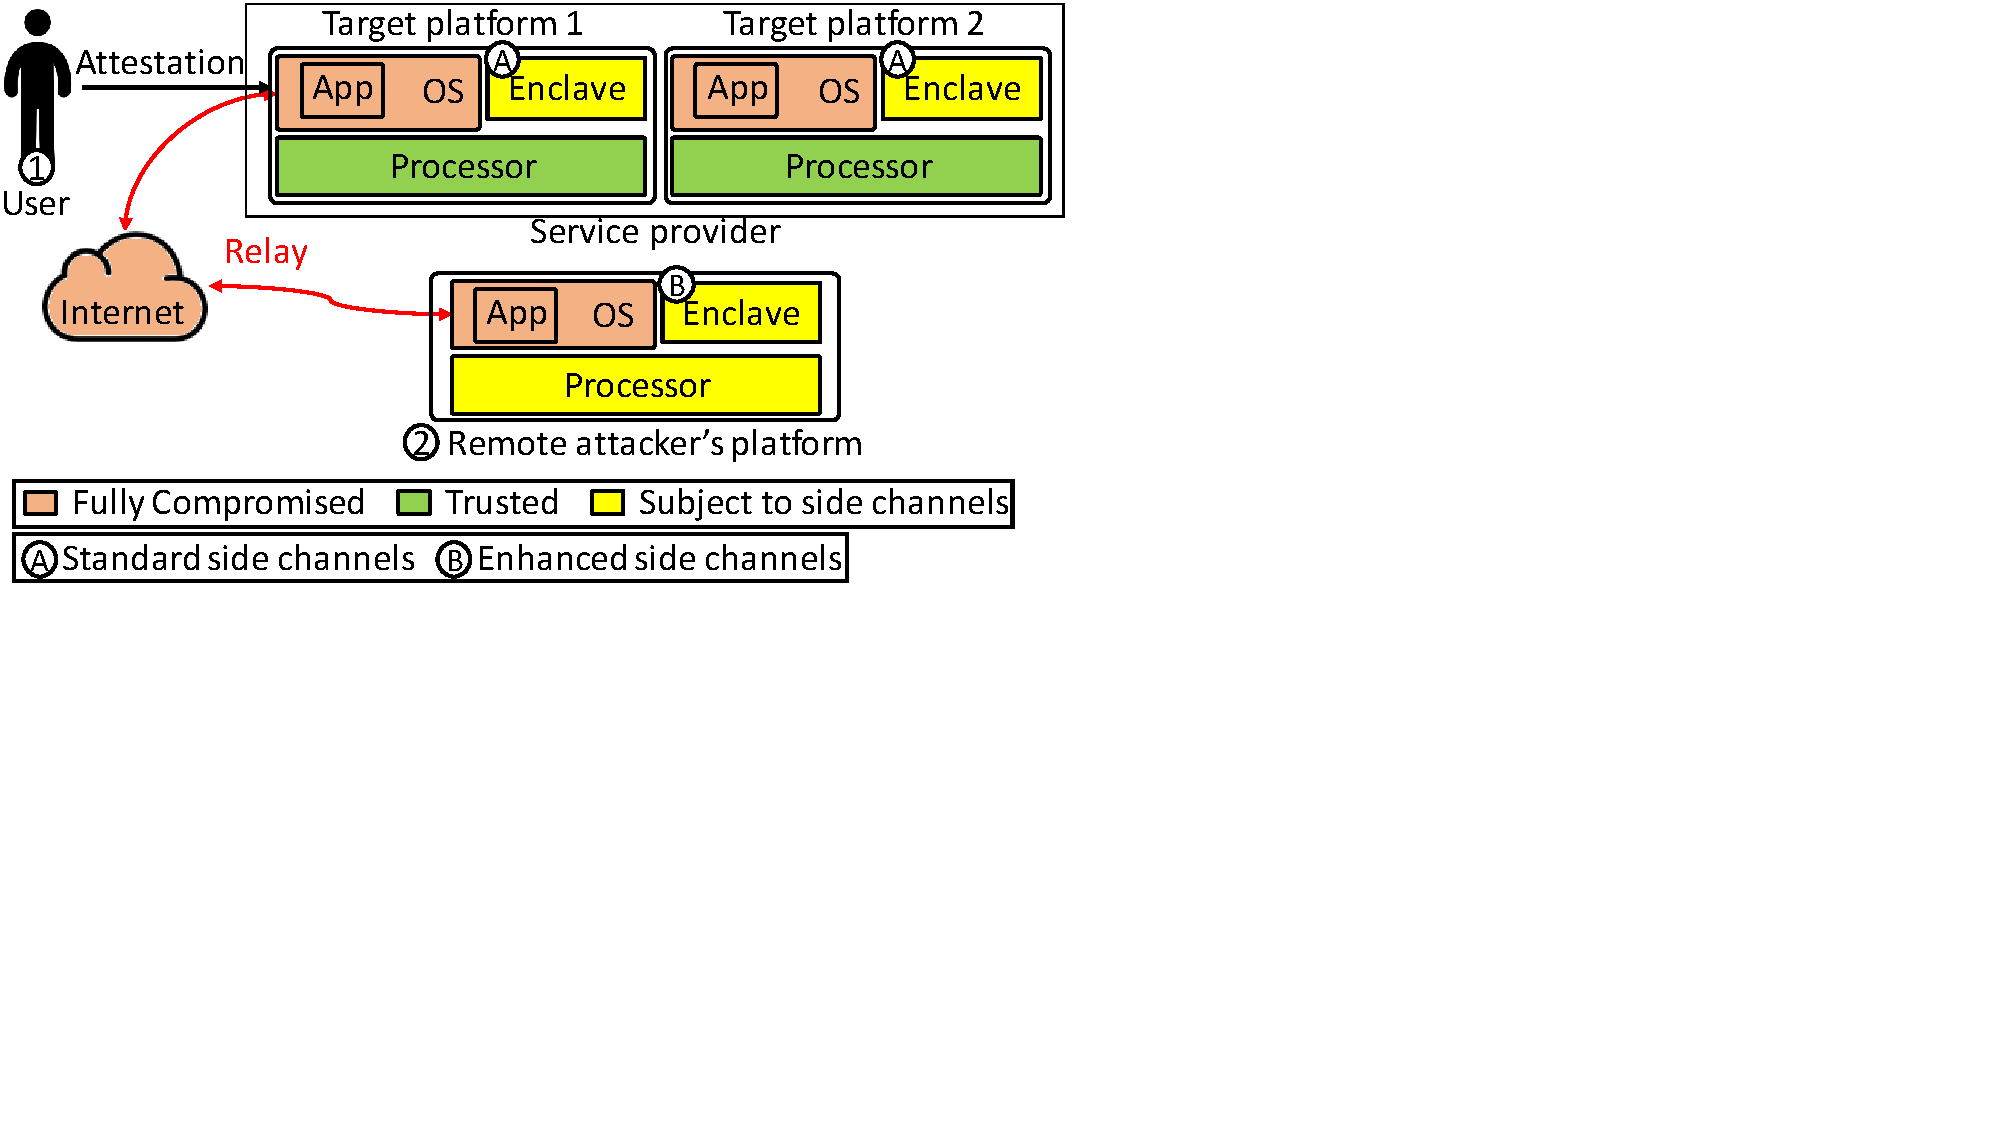
\includegraphics[trim={0cm 9cm 15.8cm 0},clip,width=0.9\linewidth]{relayAttack2.pdf}
	\caption{Attestation relay attack.}
	\label{fig:SystemModel}
\end{figure}

Unfortunately, such attestation has also a major known weakness. As shown in Figure~\ref{fig:SystemModel}, an adversary that controls the OS on the attested computing platform can easily \emph{re-direct} the attestation request to another, similar platform. The remote verifier cannot notice such \emph{relay attacks}, since the attestation mechanism is based on a group signature scheme and all processors that are part of the same group produce indistinguishable signatures. 

The problem of relay attacks have been known for a long time. Parno identified them in the context of TPM attestation over a decade ago ~\cite{parno2008bootstrapping}. However, the full implications of relay attacks are not well-understood. Since attestation can only be re-directed to another legitimate processor, it may appear that such relay attacks do not have noteworthy negative implications. Our analysis shows that such belief is misguided.

\begin{figure}[t]
\footnotesize
    \centering
    \begin{tikzpicture}[
solved/.style={rectangle,draw,fill=purple!40, rounded corners, align=center},
not/.style={rectangle, draw,fill=orange!60, rounded corners, align=center},
neutral/.style={rectangle, draw, rounded corners, align=center, fill=black!5},
sibling distance=12em]]
    \node[neutral](root) {SGX attacks}
    child { node[not, yshift=13pt] (name) {Attacks enabled by \\ leaked attestation keys ~\cite{foreshadow-usenix18}} }
    child { node[neutral, yshift=13pt] (app) {Side-Channels \\ on application enclave}
      child { node[neutral, yshift=12pt] (soft) {Software/digital}
		child { node[solved, yshift=-4pt] (pe) {Privilege\\ escalation}}      
        child { node[not, right=1.5em of pe] (a) {Complement of Case (A)}}
        child { node[solved, right=1.5em of a, yshift=-10pt] {Case (A):\\
                Target platform: secure\\
                Attacker's platform: vulnerable}}}
      child { node[solved, yshift=12pt] (physical) {Physical} } };
      
    %\node[below=0cm of name] {Foreshadow~\cite{foreshadow-usenix18}};
    \node[below=0cm of physical](power) {Power analysis}; %~\cite{wang2006covert}};
    \node[below=-5pt of power](EM) {EM radiation}; %~\cite{gandolfi2001electromagnetic}};
    \node[below=-5pt of EM](ac) {Acoustic}; %~\cite{shamir2004acoustic}};
         
    \node[left=10pt of soft](page) {Page fault}; %~\cite{xu2015controlled}};
    \node[above=-3pt of page](cache) {Cache}; %~\cite{dall2018cachequote}};
    \node[below=-2pt of page](branch) {Branch prediction}; %~\cite{lee2017inferring}};
    %\node[below=-5pt of branch](synch) {Synchronization~\cite{asyncshock}};
      
    \node[solved, right=4em of root,  minimum size=3mm](l1) {};
    \node[right=0cm of l1](l1_1) {Enabled by relay};
    \node[not, below=1pt of l1, minimum size=3mm](l2) {};
    \node[right=0cm of l2](l2_1) {Independent of relay};
    
    \end{tikzpicture}
    
    \caption{Relay attack implications.}
    \label{fig:relayTree}
\end{figure}            

\paragraph{Relay attack implications}
The main implication of relay attacks is that they \emph{increase} the adversary's ability to attack the attested enclave. As shown in Figure~\ref{fig:relayTree}, the first major benefit, from the point of view of the adversary, is that by re-direction the attestation to a platform that in the physical possession of the adversary, the adversary enables physical side-channel attacks such as acoustic, electric and electromagnetic monitoring, which have been shown to be both effective and inexpensive means to extract secrets from modern PC platforms. Hardening enclaves against physical side channels is known to be a difficult problem. 

Another benefit of relay attacks is that it may enable privilege escalation. In cases where the adversary has only compromised the user-space application that manages the enclave, and not the OS, the application can redirect the attestation to the attacker's remote platform where he controls the OS as well. In such cases, the relay enables digital side-channel attacks that require system privileges.

The third, and perhaps the most subtle, implication of relay is that it can also enable software-based side-channel attacks that would not be otherwise possible due to timing of certain events (Case(A) in Figure~\ref{fig:relayTree}). One such example is a scenario, where, at the time of attestation and secret provisioning, the enclave is hardened against all known digital side-channel attacks (e.g., using tools like Raccoon~\cite{raccoon}). After secret provisioning, the OS compromise is detected and cleaned. Later, a new side-channel attack vector (that is not prevented by the used tools) is discovered. If the adversary performed redirection and the secret was provisioned to the attacker's machine, the new side channel is exploitable. Without the relay, the attack is not possible.

Finally, we note that all attacks based on leaked attestation keys (e.g., ones obtained through the Foreshadow attack~\cite{foreshadow-usenix18}) are independent of relaying. If the adversary has obtained a valid and non-revoked attestation key, he can emulate an SGX processor on the target platform.


\subsubsection*{\proximitee System}

Our goal is to design a solution that addresses the limitations of the remote attestation Intel SGX i.e., vulnerable to the relay attack. In short, our solution should be \emph{secure} (no Trust on Fist Use (ToFU) assumption, small TCB, no online authorities) and \emph{easy to deploy} (no OS re-installation, manual configuration or pre-defined enclaves). In this section, we provide an overview of our proposed system: \proximitee.

We propose a hardened SGX attestation scheme, called \proximitee, based on a simple embedded device that we call \key. The embedded device is attached to the target platform over a local communication interface such as USB. 
Our main idea is to use the combination of such trusted device and \emph{proximity verification} to prevent relay attacks. In our solution, the \key device verifies the proximity of the attested enclave and after successful proximity verification it facilitates the creation of a secure channel between the remote verifier and the attested enclave. 

After the initial attestation, the device periodically checks proximity to the attested enclave. The established secure channel is contingent on the physical presence of the embedded device on the target machine and it stays active only as long as the device is plugged-in. The act of detaching the device automatically revokes the attested platform without any interaction with a trusted authority. Thus, our solution enables secure \emph{offline} enrollment and revocation. 

\begin{figure}[t]
 \centering
  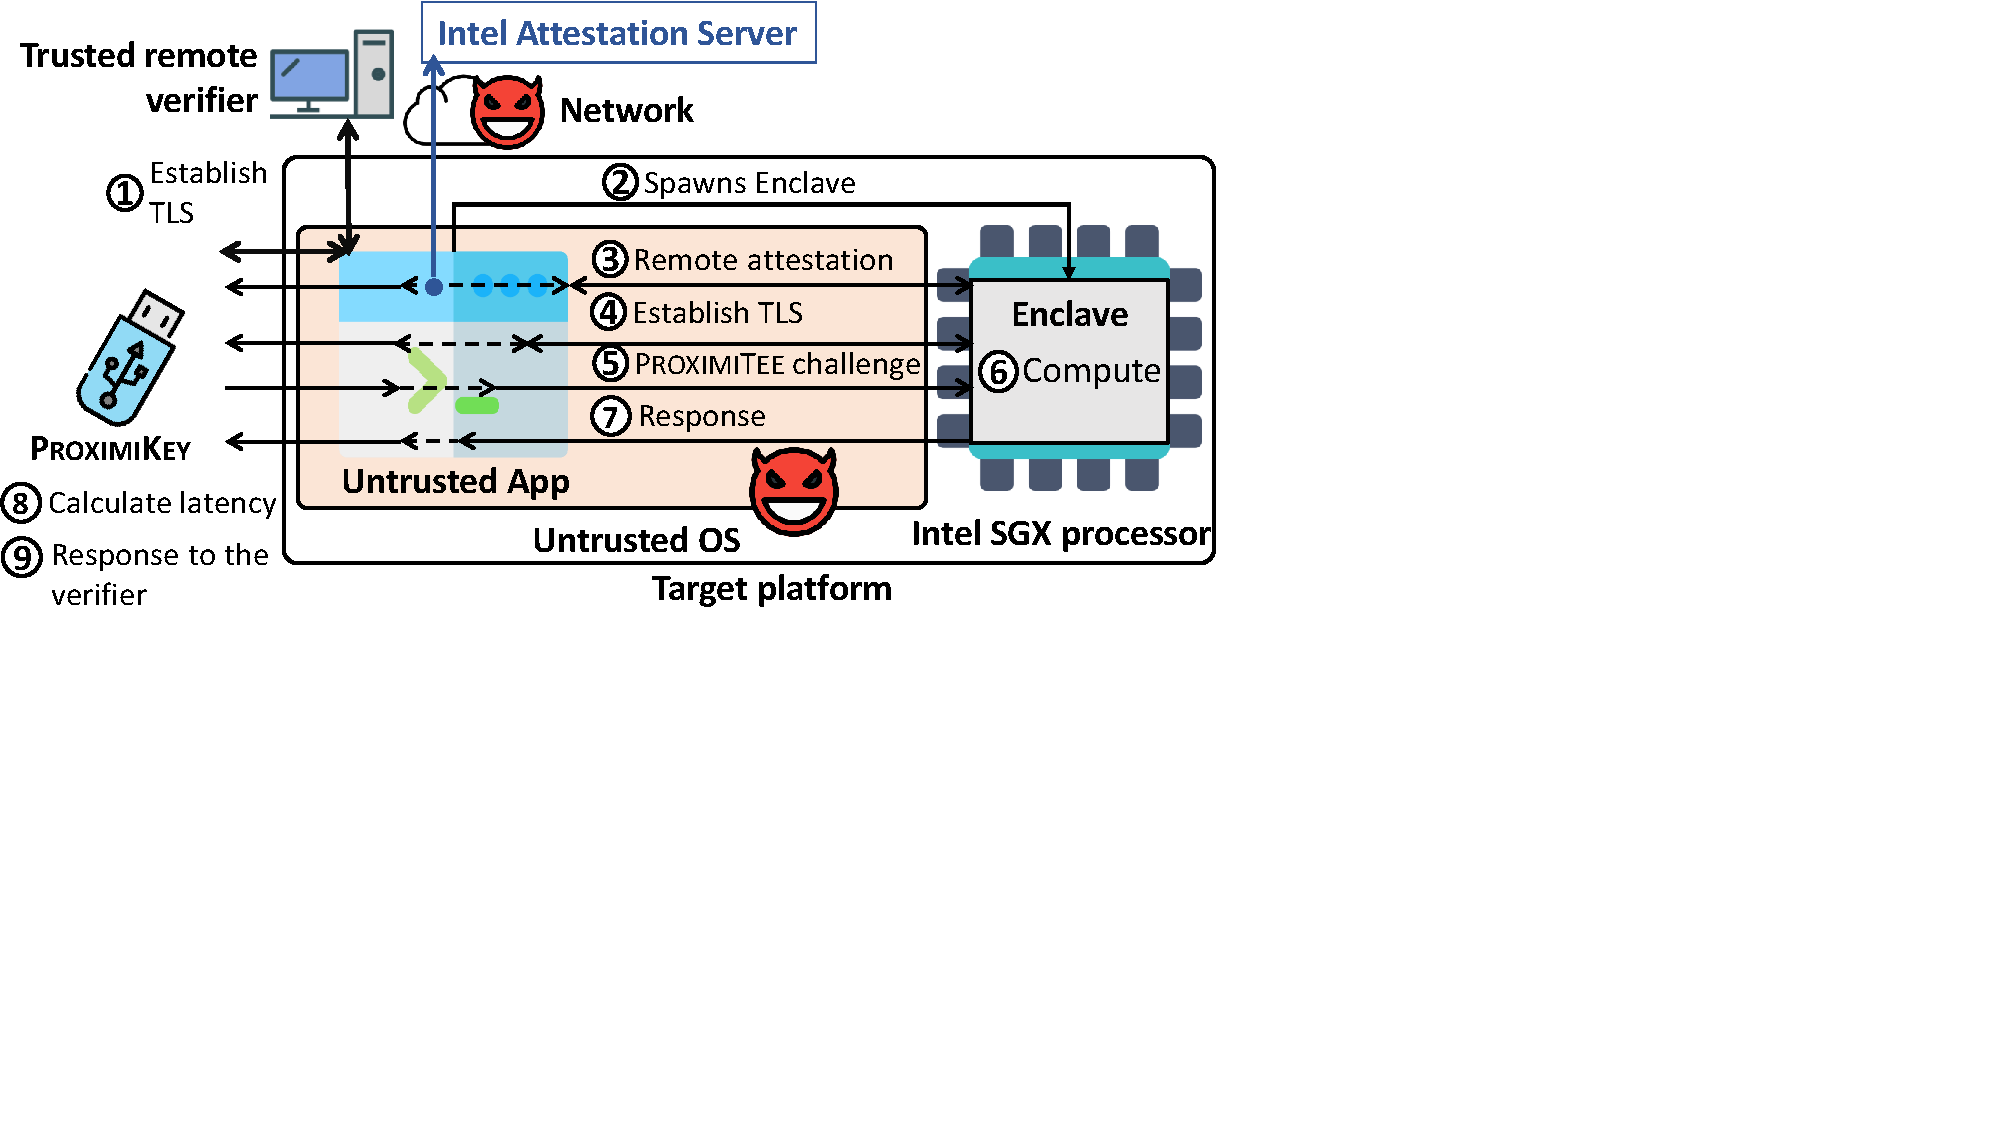
\includegraphics[trim={0 8.7cm 13.2cm 0},clip,width=\linewidth]{proximiteeMain.pdf}
 \caption{\proximitee attestation. The remote verifier establishes a secure channel to the \key device that first attests the enclave and then verifies its proximity.}
 \label{fig:systemSetUp}
\end{figure}

Figure~\ref{fig:systemSetUp} illustrates the \proximitee attestation protocol that proceeds as follows:

\begin{enumerate}
  \item[\one] The remote verifier establishes a secure channel (e.g., TLS) to the certified \key. An assisting but untrusted user-space application facilitates the connection on the target platform acting as a transport channel between the remote verifier and the \key (and later also the enclave). As part of this first step, the remote verifier specifies which enclave should be executed.

  \item[\two] The untrusted application creates and starts the attestation target enclave.

  \item[\three] \key performs the standard remote attestation to verify the code configuration of the enclave with the help of the Intel Attestation Service (IAS) Server. In the attestation protocol, the device learns the public key of the attested enclave.

  \item[\four] \key establishes a secure channel (e.g., TLS) to the enclave using that public key.

  \item[\five] \key performs a distance-bounding protocol that consists of $n$ rounds, where each round is formed by steps \five to \eight. At the beginning of each round \key generates a random challenge $r$ and sends it to the enclave over the TLS channel.

  \item[\six] The enclave increments the received challenge by one $(r+1)$.

  \item[\seven] The enclave sends a response ($r+1$) back to the \key over the TLS channel.

  \item[\eight] \key verifies that the response value is as expected (i.e., $r+1$) and checks if the latency of the response is below a threshold (\proximitee). Successful proximity verification requires that the latency is below the threshold for at least $k \times n$ responses, where $k \in (0, 1]$ is a percentage of the total number of responses $n$.

  \item[\nine] If proximity verification is successful, the \key notifies the remote verifier over the TLS channel (constructed in step \one). The verifier starts using the \key TLS channel to send messages to the enclave.
\end{enumerate}


\subsubsection*{Experiments}

We conducted our experiments on two SGX platforms and evaluate two scenarios. In one we attach the \key to one of the platform to evaluate the round trip time between the \key and an enclave running on the attached platform. This serves as the base case where no relay attack takes place. In another scenario, we connect the two SGX platforms over a 1m long Ethernet wire ro evaluate the round trip time between two enclaves running on these platforms -- simulating the relay attack.

\begin{figure}[t]
  \centering
    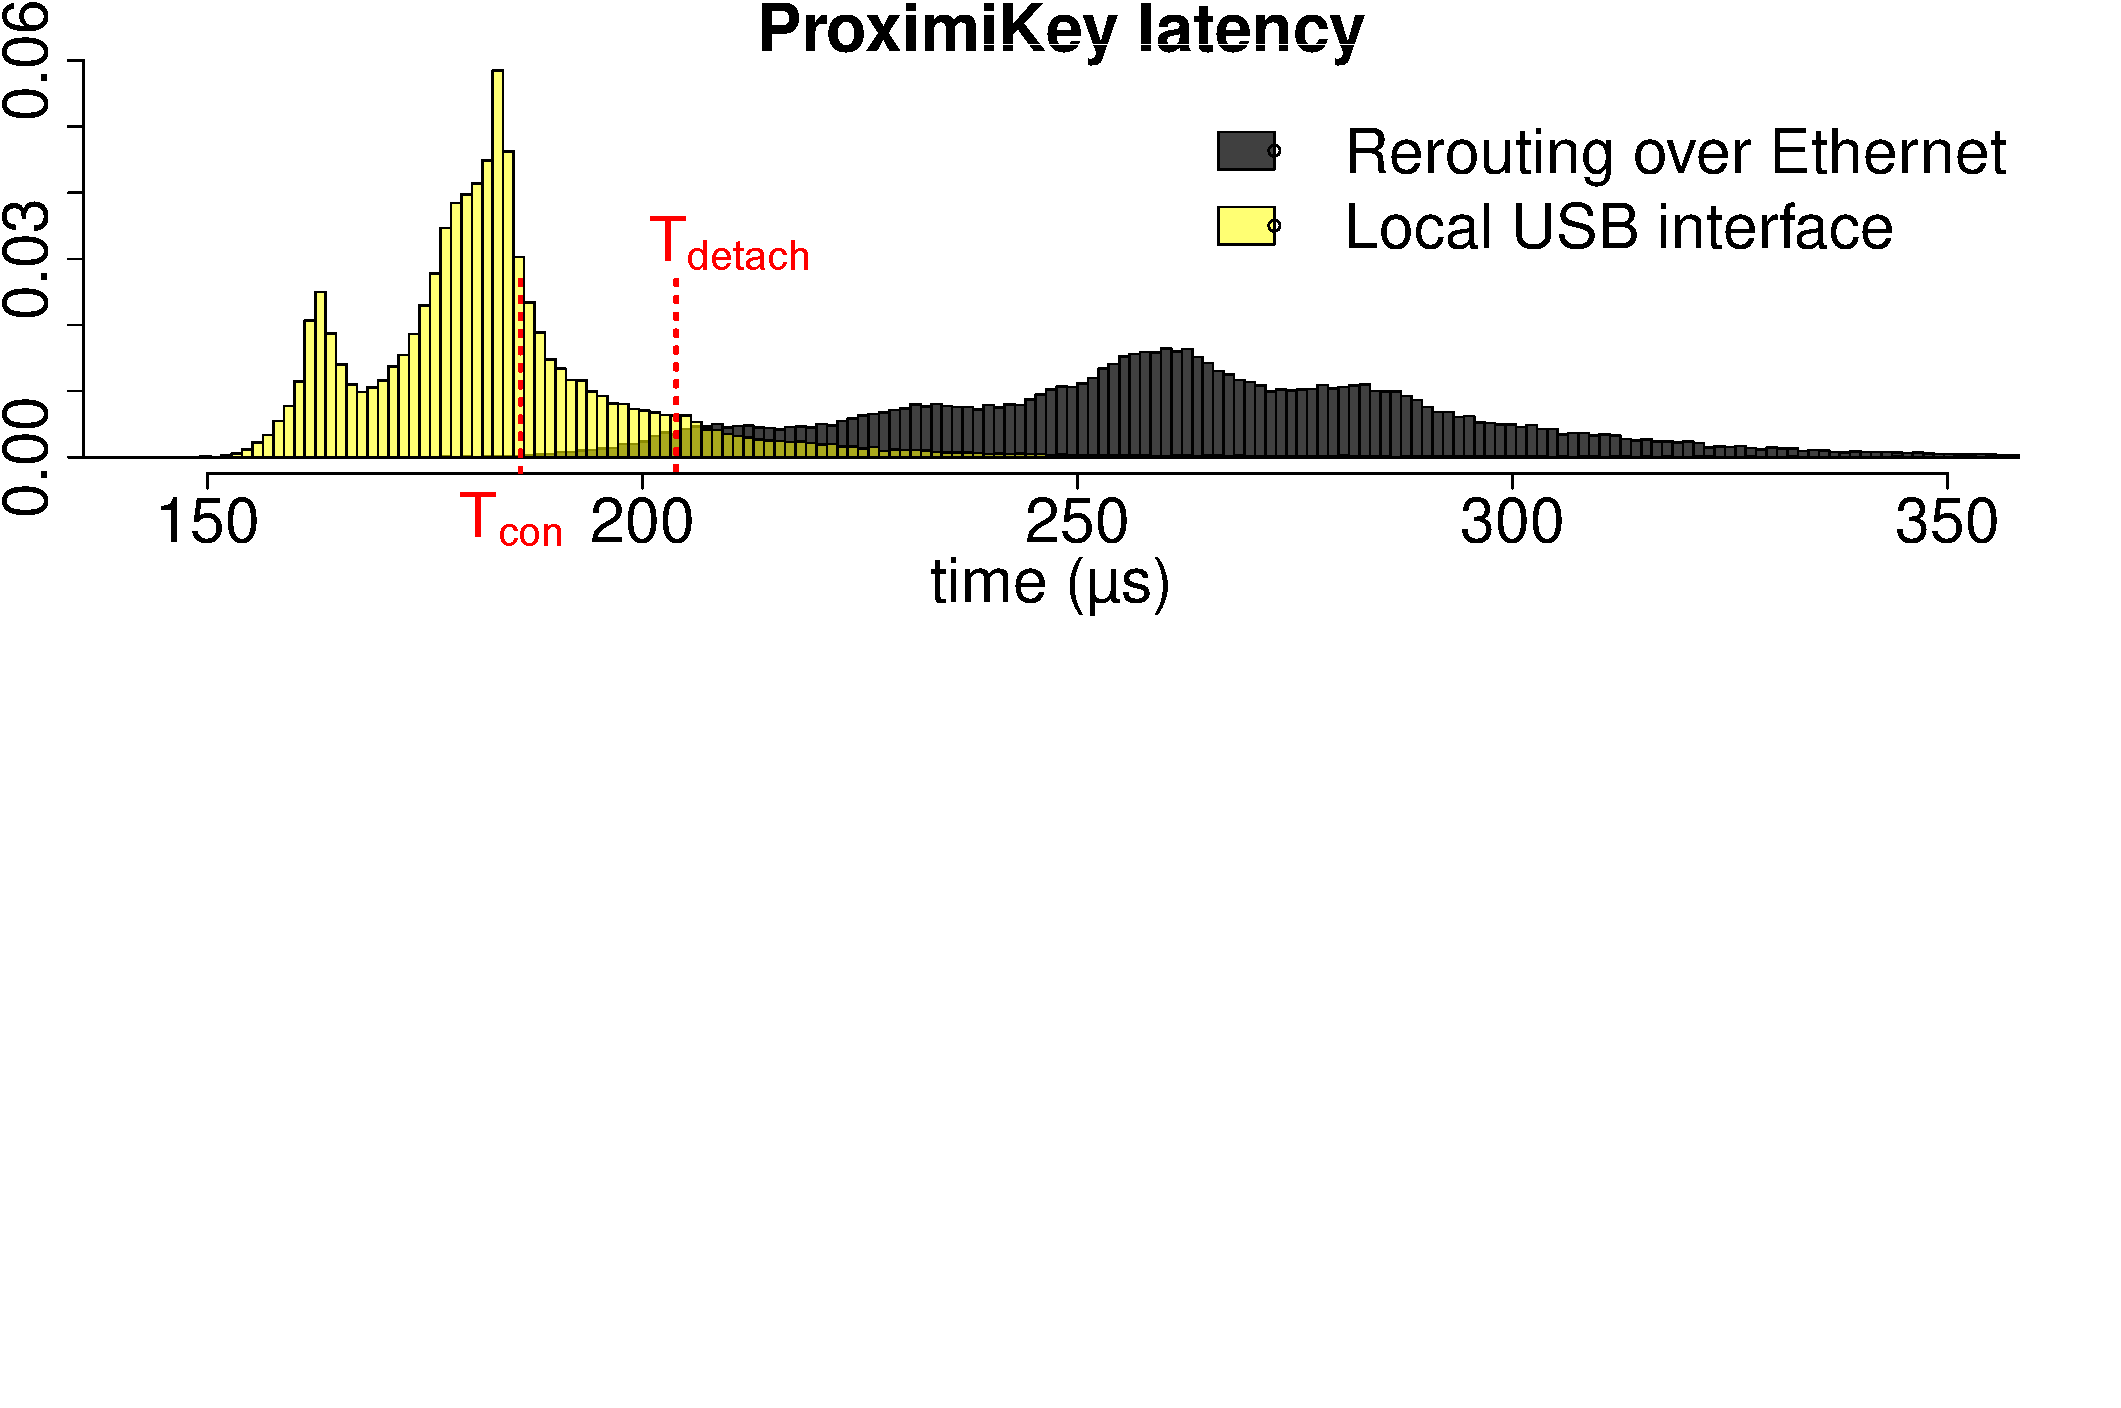
\includegraphics[trim={0 13.4cm 0 0},
    clip,width=\linewidth]{histo.pdf} 
    \caption{Latency distributions for legitimate challenge-response rounds and simulated relay attack.}
    \label{graph:instatAttackerHisto}
\end{figure}

The histogram in Figure~\ref{graph:instatAttackerHisto} on the left represents the challenge-response latencies in the legitimate proximity verification. The histogram on the right shows latencies in a simulated attack (including a post-processing phase where we reduce the adversary's measured network latencies to half to accommodate the assumption of the attacker's infinitely fast network interface).

As can be seen from Figure~\ref{graph:instatAttackerHisto}, the vast majority of the benign challenge-responses take from $145$ to $250 \mu s$. The vast majority of the round-trip times in the simulated attack take from $200$ to $750$ $\mu s$. Hence, the average delay of our simulated adversary is only $80 \mu s$. To put this into perspective, even the highly-optimized network connections between major data centers in the same region exhibit latencies from one millisecond upwards which is one order of magnitude more than in our simulated setup.

We simulate a powerful relay-attack adversary that is connected to the target platform with fast network connection. To consider the best case for the adversary, we make several assumptions in his favor. For example, we assume that he can instantly perform all computations needed to participate in the proximity verification protocol. However, he cannot break cryptographic hardness assumptions. We define the adversary's success as the event in which proximity verification succeeds with an enclave that resides on the attacker's platform and denote the probability of such event $P_{adv}$. We define the legitimate success as the event in which proximity verification succeeds with an enclave that resides in the target platform and denote its probability $P_{legit}$. We saw that it is possible to find parameters ($n=50$, $k=0.3$ and \proximitee$=186 \mu s$) that make proximity verification very secure ($P_{adv}=3.55\times 10^{-34}$) and reliable ($P_{legit}=0.999999977$).




